\documentclass[12pt]{report}
\usepackage[utf8x]{inputenc}
\usepackage{amsmath}
\usepackage{amsfonts}
\usepackage{mathrsfs}
\usepackage{natbib}
\usepackage{graphicx} % figuras
%\usepackage[export]{adjustbox} % loads also graphicx
\usepackage{float}
\usepackage[font=footnotesize]{caption}
\usepackage{wrapfig}
%\usepackage{authblk}
%\usepackage{subfigure}
\usepackage{pifont}
\usepackage{a4wide}
\usepackage{wrapfig}
 \usepackage{tabu}
%\usepackage{multirow}% 

%\graphicspath{/home/wagm/cortes/Localdisk/Results/16_05/05_09/}
\topmargin=-2pt
\title{Physics-based pre-conditioners for large-scale subsurface flow simulation}

%\author[1]{G. B. Diaz Cortes}  
%\author[1]{C. Vuik} 
%\author[2]{J. D. Jansen} 
%\affil[1]{Department of Applied Mathematics, TU Delft}
%\affil[2]{Department of Geoscience \& Engineering, TU Delft}
%\renewcommand\Authands{ and }
%\date{March 2016}
\begin{document}
\thispagestyle{empty}
% \noindent
% \begin{center}
% {\Large \sc DELFT UNIVERSITY OF TECHNOLOGY}
% \\
% \vspace{3cm}
% {\large \sc REPORT 16-03}\\[4ex]
% {\large \sc Physics-based pre-conditioners for large-scale subsurface flow simulation}\\[4ex]
% {\large \sc G. B. Diaz Cortes, C. Vuik, J. D. Jansen}\\
% \vfill
% {\tt ISSN 1389-6520}\\[2ex]
% {\tt Reports of the Delft Institute of Applied Mathematics}\\[2ex]
% {\tt Delft 2016}
% \end{center}
% \pagebreak
% \thispagestyle{empty}
% \vspace*{\fill}
% \noindent
% \hspace*{-0,3cm}Copyright~~~\Pisymbol{psy}{227}~~~2016 by Delft Institute of Applied Mathematics, Delft, \mbox{The Netherlands.}
% \\[2ex]
% No part of the Journal may be reproduced, stored in a retrieval system, or
% transmitted, in any form or by any means, electronic, mechanical, photocopying,
% recording, or otherwise, without the prior written permission from Delft Institute of
% Applied Mathematics, Delft University of Technology, The
% Netherlands. 
% % newpage, title etc.
% \setcounter{page}{1}


% Title Page

%\maketitle
 \section*{Compressible problem}
To describe single-phase flow through a porous medium, we use the continuity equations:
\begin{equation}\label{eq:ce}
\frac{\partial (\rho \phi)}{\partial t}+ \nabla \cdot ( \rho \mathbf{v})=q, \qquad \mathbf{v}=-\frac{\mathbf{K}}{\mu}(\nabla \mathbf{p}-\rho g\nabla z),
\end{equation}
or
\begin{equation}\label{eq:ce1}
\frac{\partial (\rho \phi)}{\partial t}- \nabla \cdot \left( \frac{\rho\mathbf{K}}{\mu}(\nabla \mathbf{p}-\rho g\nabla z)\right)=q.
\end{equation}
Where the primary unknown is the pressure $\mathbf{p}$ and the fluid  $\rho=\rho(\mathbf{p})$ and rock $\phi=\phi(\mathbf{p})$ compressibilities can be pressure dependent.
Rock compressibility is defined by:
\begin{equation*}
 c_r=\frac{1}{\phi}\frac{d\phi}{dp}=\frac{ln(\phi)}{dp},
\end{equation*}
If the rock compressibility is constant, the previous equation can be integrated as:
\begin{equation*}
 \phi(p)=\phi_0 e^{c_r(p-p_0)}.
\end{equation*}
Fluid compressibility is defined as:
\begin{equation}\label{eq:fc}
 c_f=\frac{1}{\rho}\frac{d\rho}{dp}=\frac{ln(\rho)}{dp}.
\end{equation}
If the fluid compressibility is constant, the previous equation can be integrated as:
\begin{equation}\label{eq:rhoeq}
 \rho(\mathbf{p})=\rho_0 e^{c_f(\mathbf{p}-\mathbf{p}_0)}.
\end{equation}
Well model\\
The relation between the bottom-hole pressure and the surface flow rate in a well is given by the 
the linear law:
$$q_0=J(p_R-p_{bhp}),$$
where $J$ is the productivity or injectivity index, in MRST
$$q_{j}=W_j(p_{r,j}-p_{bhp,j}).$$\\
Using implicit discretization, Equation \eqref{eq:ce} becomes:
\begin{equation}\label{eq:ce2}
 \frac{(\mathbf{\phi}\mathbf{\rho})^{n+1}-(\mathbf{\phi}\mathbf{\rho})^{n}}{\Delta t^n}
 +\nabla \cdot (\mathbf{\rho} \mathbf{v})^{n+1}=\mathbf{q}^{n},
\qquad
\mathbf{v}^{n+1}= -\frac{\mathbf{K}}{\mu^{n+1}}[\nabla(\mathbf{p}^{n+1})-g\mathbf{\rho}^{n+1}\nabla(\mathbf{z})].
\end{equation}
If $\mathbf{\phi}$ and $\mathbf{\rho}$ depend nonlinearly on $\mathbf{p}$ we have a nonlinear system 
of equations to be solved for each time step.  \\
Assuming no gravity terms, Equation \eqref{eq:ce}
can be rewritten as:
\begin{equation}\label{eq:ce3}
 \frac{\mathbf{\phi}(\mathbf{p}^{n+1})\mathbf{\rho}(\mathbf{p}^{n+1})
 -\mathbf{\phi}(\mathbf{p}^{n})\mathbf{\rho}(\mathbf{p}^{n})}{\Delta t^n}
 +\nabla \cdot (\mathbf{\rho} \mathbf{v})^{n+1}=\mathbf{q}^{n},
\qquad
\mathbf{v}^{n+1}= -\frac{\mathbf{K}}{\mu^{n+1}}\nabla(\mathbf{p}^{n+1}).
\end{equation}
Or:
\begin{equation}\label{eq:ce4}
 \frac{\mathbf{\phi}(\mathbf{p}^{n+1})\mathbf{\rho}(\mathbf{p}^{n+1})
 -\mathbf{\phi}(\mathbf{p}^{n})\mathbf{\rho}(\mathbf{p}^{n})}{\Delta t^n}
 -\nabla \cdot (\mathbf{\rho}(\mathbf{p}^{n+1}) 
 \frac{\mathbf{K}}{\mu^{n+1}}\nabla(\mathbf{p}^{n+1}))-\mathbf{q}^{n}=0.
\end{equation}
The latter system can be written in short vector form as:
\begin{equation}\label{NR}
 \mathbf{F}(\mathbf{p}^{n+1};\mathbf{p}^n)=0,
\end{equation}
with $\mathbf{p}^n$ the vector of unknown state variables at the time step $n$.\\
This non-linear system can be solved by Newton's method, the $(i+1)$-th iteration approximation is obtained from:
$$\frac{\partial \mathbf{F}(\mathbf{x}^i)}{\partial \mathbf{x}^i}\delta\mathbf{x}^i=-\mathbf{F}(\mathbf{x}^i),
\qquad \mathbf{x}^{i+1}=\mathbf{x}^i+\delta \mathbf{x}^{i+1},$$
where $\mathbf{J}(\mathbf{x}^i)=\frac{\partial \mathbf{F}(\mathbf{x}^i)}{\partial \mathbf{x}^i}$ is the 
Jacobian matrix, and $\delta \mathbf{x}^{i+1}$ is the Newton update at iteration step $i+1$.\\
\section*{MRST}
The MRST (MATLAB Reservoir Simulation Toolbox) allows the use of various grid types, which are stored using a general unstructured
format, in which cells, faces, vertices's and connections between cells and faces are explicitly
represented. \\
There is a wide range of structured and unstructured grids that can be constructed in MRST.
For the structured grids, a pattern is chosen and repeated. The most typical structured grids are 
based on quadrilaterals in 2D and hexahedral 3D.

\subsubsection{Cartesian grids.}
The simplest structured grid is based in a square in 2D and a cube in 3D. to construct these
grids in the MRST we need to specify the domain $[0\: Lx,\: 0\: Ly]$ represented as $[Lx\: Ly]$, and
number of cells $nx, ny$, for cartesian grids the construction is in the next form:\\
$$
G\:=\:cartGrid([nx,ny],[Lx,Ly]) \qquad 2D, $$
$$G\:=\:cartGrid([nx,ny],[Lx,Ly,Lz]) \qquad 3D.
$$



\subsubsection{Rectilinear grids.}
These are also called tensor grids, are rectilinear shapes (rectangles or parallelepipeds) not necessarily 
congruent to each other.\\
\begin{figure}[h!]
\centering
\begin{minipage}{.6\textwidth}
 \centering
\includegraphics[width=6cm,height=6cm,keepaspectratio]{/home/wagm/cortes/Desktop/work/writing/pics/cartGrid3d.jpg}
\caption{Cartesian grid in 3D.}
\label{fig:Cartgrid3D}
\end{minipage}%
\begin{minipage}{.5\textwidth}
\centering
\includegraphics[width=6cm,height=6cm,keepaspectratio]{/home/wagm/cortes/Desktop/work/writing/pics/rectGrid2d.jpg}
\caption{Rectangular grid in 2D.}
\label{fig:Rectgrid2D}
\end{minipage}
\end{figure}
The grid structure contains three fields: cells, faces and nodes that specify the individual properties of
each cell/face/vertex in the grid.
The cell structure, G.cells, contains the following fields:
\begin{itemize}
 \item num: the number $n_c$ of cells in the global grid.
\item facePos: an indirection map of size [num+1,1] into the faces array. Specifi-
cally, the face information of cell i is found in the submatrix
faces(facePos(i) : facePos(i+1)−1, :)
The number of faces of each cell may be computed using the state-
ment diff(facePos) and the total number of faces is given as nf =
facePos(end)−1.
\item  faces: an $n_f\times3$ array that gives the global faces connected to a given cell.
If faces(i,1)==j, the face with global number faces(i,2) is
connected to cell number j. The last component, faces(i,3), is optional
and can for certain types of grids contain a tag used to distinguish face
directions: East, West, South, North, Bottom, Top.
\item indexMap: an optional $n_c \times 1$ array that maps internal cell indices to external
cell indices. For models with no inactive cells, indexMap equals 1 : nc . For
cases with inactive cells, indexMap contains the indices of the active cells
sorted in ascending order. 
\end{itemize}
The face structure, G.faces, consists of the following mandatory fields:
\begin{itemize}
 \item num: the number $n_f$ of global faces in the grid.
 \item nodePos: an indirection map of size [num+1,1] into the nodes array. 
 The node information of face i is found in the submatrix
nodes(nodePos(i) : nodePos(i+1)−1, :)
The number of nodes of each face may be computed using the state-
ment diff(nodePos). Likewise, the total number of nodes is given as $nn =
nodePos(end)−1$.
\item nodes: an $N_n \times 2$ array of vertices in the grid. If nodes(i,1)==j, the local
vertex i is part of global face number j and corresponds to global vertex nodes(i,2). 
For each face the nodes are assumed to be oriented such
that a right-hand rule determines the direction of the face normal. As
for cells.faces, the first column of nodes is redundant and can be easily
reconstructed. 
\item  neighbors: an $n_f \times 2$ array of neighboring information. Global face i is
shared by global cells neighbors(i,1) and neighbors(i,2). One of the entries
in neighbors(i,:), but not both, can be zero, to indicate that face i is an
external face that belongs to only one cell (the nonzero entry).

\end{itemize}

\newpage
To solve this problem with MRST, it is necessary to define the equations and some operators. \\
Assuming no-flow boundary conditions, the equations are defined only for the interior faces of the grid.
The MRST function $computeTrans$ computes the half transmissibilities associated 
with the two-point flux approximation (TPFA). Then, it is necessary to compute the harmonic average to 
obtain the face-transmissibilities. 
For neighboring cells, this is $T_{ij}=(T_{i,j}^{-1}+T_{j,i}^{-1})^{-1}$.\\
The divergence and gradients are defined as discrete functions. Taking N as the interior faces, 
the gradient of a vector $\mathbf{x}$ is defined as:
$$grad(\mathbf{x})=\mathbf{x}(N(:,2))-\mathbf{x}(N(:,1))=\mathbf{C}\mathbf{x},$$
where $N(:,1)$ and $N(:,1)$ are the Neighboring faces. The divergence function is the negative 
transpose of the $grad$ function.
$$div(\mathbf{x})=-\mathbf{C'}\mathbf{x}.$$
To model flow through a porous medium with MRST, we need to define the equation for the pressures, 
the equations for the mass flow rates at the wells and the
control equations for the wells. To define this equations, first we have to define the equations
that relate the pressure with the density and the porosity. In this first cases, we will set
the rock compressibility as zero, therefore, only the equation for the density is defined.
\begin{table}[H]
\centering
{\tabulinesep=1.11mm \begin{tabu}{ |l |} 
\hline
$c=1e-3/bars$\\
$rho_r= 850*kilogram/meter ^  3$\\
$rho=@(p) rho_r.*exp(c*p-p_r)$\\
 \hline
\end{tabu}}
\label{table:rh}
\end{table} 
Darcy's law \eqref{eq:ce3} for each face $f$ in MRST is written as:
$$\mathbf{v}[f]=-\frac{\mathbf{T}[f]}{\mu}grad(p),$$
and the continuity equation for each cell $c$:
$$\frac{1}{\Delta t}\left((\phi(\mathbf{p})[c]\rho(\mathbf{p})[c])^{n+1}-(\phi(\mathbf{p})[c]\rho(\mathbf{p})[c])^{n}\right)
+div(\rho_a\mathbf{v})[c]=\mathbf{0},$$
where $\rho_a$is the arithmetic average of the density.
In MRST, the latter equations are implemented as anonymous functions of pressure:
$$v= @(p)\quad (T/mu).*grad(p),$$
\begin{equation}\label{eq:pressEq}
pressEq= @(p,p_0,dt) \quad(1/dt)(pv(p).*rho(p)-pv(p0).*rho(p0))+div(avg(rho(p)).*v(p)),
\end{equation}
where $p_0$ is the pressure at the previous time step, and $p$ is the pressure at the current time step.\\ 
The sources in this problem are wells, each cell where the well is connected to the reservoir is called
connection. In MRST $wc$ are the connection grid cells, $WI$ are the well indices and $dz$ is the depth
relative to bottom-hole. \\
In presence of gravity, we need to consider the hydrostatic pressure drop (in this case we assume no gravity, so is not necessary).
Assuming the fluid density in the well as constant, the pressure $\mathbf{p}[N_c(w)]$ in connection w
of well $N_w(w)$ is given by:
$$\mathbf{p}_c[w]=\mathbf{p}_{bh}[N_w(w)]+g \Delta z[w]\rho(\mathbf{p}_{bh}[N_w(w)]),$$
where $\Delta z[w]$ is the vertical distance from bottom-hole to the connection, 
$$p_{conn}=@(bhp)\quad bhp+g*dz.*rho(bhp).$$
The pressure at the well connection is related to the average 
pressure inside the grid cell by the Peaceman model. With this model, the mass flow rate at connection c 
is given by:
$$q_c[w]=\frac{\rho(\mathbf{p}[N_c(w)])}{\mu}WI[w](\mathbf{p}_c[w]-\mathbf{p}[N_c(w)]),$$
where $\mathbf{p}[N_c(w)]$ is the pressure in the cell $N_c(w)$ surrounding connection w,
$$q_{conn}=@(p,bhp) \quad WI.*(rho(p(wc))/mu).*(p_{conn}(bhp)-p(wc)).$$
The volumetric well-rate at surface conditions is obtained summing up all the mass well rates and dividing by the 
surface density:
\begin{equation}\label{eq:rateEq}
 rateEq=@(p,bhp,qS) \quad qS-sum(q_{conn}(p,bhp))/rhoS,
\end{equation}
where the free variables are p, bhp and qS. To control the well we need an equation to specify 
the bottom-hole pressure ($p_{bhp}$):
\begin{equation}\label{eq:ctrlEq}
 ctrlEq=@(bhp)\quad bhp-p_{bhp}.
\end{equation}
Once that the equations are defined for $p$ (Equation \eqref{eq:pressEq}), $bhp$ (Equation \eqref{eq:ctrlEq})
and $qS$ (Equation \eqref{eq:rateEq}), the variables are initialized for automatic differentiation (see Appendix \ref{a1})
with the initial values, which gives as result:
\begin{table}[H]
\centering
{\tabulinesep=1.11mm \begin{tabu}{ |c c |} 
\hline
$\mathbf{p}_{ad}$= ADI Properties:  & $bhp_{ad}$= ADI Properties: \\
  val: $\mathbf{p}_{init}$ & val: $p(wc)_{init}$ \\ 
  jac: $\{[\frac{\partial \mathbf{p}}{\partial \mathbf{p}}=\mathbf{I}]$   $[\frac{\partial \mathbf{p}}{\partial p_{bh}}=0]$  $[\frac{\partial \mathbf{p}}{\partial qS}=0]\}$&
  jac: $\{[\frac{\partial p_{bh}}{\partial \mathbf{p}}=\mathbf{0}]$   $[\frac{\partial p_{bh}}{\partial p_{bh}}=1]$  $[\frac{\partial p_{bh}}{\partial qS}=0]\}$\\
&\\
\multicolumn{2}{|c|}{$qS_{ad}$= ADI Properties:}\\ 
\multicolumn{2}{|c|}{val: $0$}\\  
\multicolumn{2}{|c|}{ jac: $\{[\frac{\partial qS}{\partial \mathbf{p}}=\mathbf{0}]$   $[\frac{\partial qS}{\partial p_{bh}}=0]$  $[\frac{\partial qS}{\partial qS}=1]\}$}\\ 
 \hline
\end{tabu}}
\label{table:1}
\end{table} 
These results are stored in a single matrix that contains sub-matrices with the jacobians of the variables.
The jacobian matrix of the full system (eq) is the next one:
\begin{table}[H]
\centering
{\tabulinesep=1.11mm \begin{tabu}{ |c c c |} 
\hline
$eq\{1\}.jac\{1\}=\frac{\partial \mathbf{p}}{\partial \mathbf{p}}$ & $eq\{1\}.jac\{2\}=\frac{\partial \mathbf{p}}{\partial p_{bh}}$
&$eq\{1\}.jac\{3\}=\frac{\partial \mathbf{p}}{\partial qS}$\\

$eq\{2\}.jac\{1\}=\frac{\partial p_{bh}}{\partial \mathbf{p}}$ &  $eq\{2\}.jac\{2\}=\frac{\partial p_{bh}}{\partial p_{bh}}$&  
$eq\{2\}.jac\{3\}=\frac{\partial p_{bh}}{\partial qS}$\\

$eq\{3\}.jac\{1\}=\frac{\partial qS}{\partial \mathbf{p}}$ &  $eq\{3\}.jac\{2\}=\frac{\partial qS}{\partial p_{bh}}$ &
$eq\{3\}.jac\{3\}=\frac{\partial qS}{\partial qS}$\\ 
 \hline
\end{tabu}}
\label{table:2}
\end{table}  
From this matrix, we can obtain the jacobian and the residual for the Newton-Raphson iteration. Once the 
jacobian is obtained, the solution can be computed.
\begin{table}[!ht]
\centering
{\tabulinesep=1.11mm \begin{tabu}{ |c |} 
\hline
$\mathbf{J}=eq.jac\{1\}$   \%Jacobian\\
$res=eq.val$   \%residual\\
$upd=-(\mathbf{J}/res)$   \%Newton update\\
 \hline
\end{tabu}}
\label{table:2}
\end{table}

The algorithm is presented below:\\
\begin{table}[!ht]
{\tabulinesep=1.11mm \begin{tabu}{ |l |} 
\hline
  \textbf{Algorithm 1} \\
  \hline
 \hline
\\
$numSteps = 52$ \% number of time−steps\\
$totTime = 365*day$ \% total simulation time\\
$dt = totTime$ / numSteps \% constant time step\\
$tol = 1e−5$ \% Newton tolerance\\
$maxits = 10$ \% max number of Newton its\\
\\
$t = 0$\\ $step = 0$ \%initialize time and steps\\
$[p_{ad},bhp_{ad},qS_{ad}]=initVariableADI(p_{init},p(wc)_{init},0)$  \hspace{1cm} \%initialize variables\\
\\
\hspace{0.5cm}\textbf{while} t $<$ totTime\\
 \hspace{1cm} $t = t + dt$\\ 
 \hspace{1cm}$step = step + 1$\\
  \hspace{1cm}\% Newton loop \\
 \hspace{1cm} $resNorm = 1e99$\\
 \hspace{1cm} $p0 = double(p_{ad})$ \hspace{2cm}\% Previous step pressure\\
 \hspace{1cm} $nit = 0$\\ \\
 \hspace{1cm} \textbf{while} (resNorm $>$ tol) \&\& (nit $<=$ maxits)\\
 \hspace{1.5cm}  \% Newton update\\
 \hspace{2cm}  $\mathbf{J}=eq.jac\{1\}$ \hspace{1.5cm}  \%Jacobian\\
\hspace{2cm}$res=eq.val$  \hspace{2cm} \%residual\\
\hspace{2cm}$upd=-(\mathbf{J}/res)$ \footnote[1]{}   
\hspace{1.5cm}\%Newton update, the solution of this system\\
\hspace{7cm}is obtained with ICCG or DICCG\\
  \hspace{1.5cm}  \% Update variables\\
\hspace{2cm}$p_{ad}.val+upd(pIx)$ \\
\hspace{2cm}$bhp_{ad}.val+upd(bhpIx)$  \\
\hspace{2cm}$qS_{ad}.val+upd(qsIx)$   \\
\hspace{2cm} resNorm = norm(res) \footnote[2]{}\\
  \hspace{1.5cm}  $nit= nit + 1$\footnote[3]{}\\
\hspace{1cm} \textbf{end}\\
\hspace{0.5cm}\textbf{end}\\
\hline
\end{tabu}}
\end{table}
\newpage
[1] Note that the update is computed 
without taking into account the norm of the residual ($resNorm$) for each time step . If the solution is reached
in the previous time step, it won't be taken into account and the first update will be computed.
[2] Only when the variables are already updated, the residual is computed. At this point, the number 
of iterations for the NR method is 0, it is only updated [3] after the first computation of the residual, 
when a first update has already be done.\\

For the solver the two algorithms are presented below:\\
\begin{table}[!h]
\begin{tabular}{ |l | } 
\hline
  \textbf{Algorithm 2. ICCG} \\
  \hline
 \hline
\\
Select $x_0$ \% It is random for the first time step\\
\hspace{1.7cm} \% and the solution of the previous time step for the rest\\
Compute $r_0=b-Ax_0$ \% the residual\\
Solve $Mr_0=r_0$  \% in this case $M= l^T l$ then we need to solve $r_0=l \backslash r_0$ \\
Solve $M^{-T}r_0=p_0$  \% in this case $M= l^T l$ then we need to solve $p_0=l^{T} \backslash r_0$ \\
$nb=norm(M^{-1}b)$  \% for the stopping criteria, we need to compute the \\
\hspace{2.5cm} 2-norm of the preconditioned right hand side \\
$tol = 1e−7$ \% Tolerance\\
\\
\hspace{0.5cm}\textbf{for} $j=0,...,$ until convergence\\
 \hspace{1cm} $w_j=Ap_j;$\\ 
 \hspace{1cm}$\alpha_j=\frac{(r_j,r_j)}{(p_j,w_j)}$\\
 \hspace{1cm} $x_{j+1}=x_j+\alpha_jp_j$\\
 \hspace{1cm} $r_{j+1}=r_j-\alpha_j*(l\backslash w_j)$ \\
 \hspace{1cm} $\beta_j=\frac{(r_{j+1},r_{j+1})}{(r_j,r_j)}$\\ 
 \hspace{1cm} $p_{j+1}=l^{T}\backslash r_{j+1}+\beta_jp_j$ \\
\hspace{1cm} $rr=\frac{(r_{j+1},r_{j+1})}{nb}$ \%Compute the relative residual\\
\hspace{4cm} and if it is smaller than the tolerance stop\\
\hspace{4cm} $\frac{||l^{-1}r||_2}{||l^{-1}b||_2}$\\
\hspace{0.5cm}\textbf{end}\\
\hline
\end{tabular}
\end{table}
\begin{table}[!h]
\begin{tabular}{ |l | } 
\hline
  \textbf{Algorithm 3. DICCG} \\
  \hline
 \hline
\\
Select $x_0$ \% It is random for the first time step\\
\hspace{1.7cm} \% and the solution of the previous time step for the rest\\
Compute $r_0=b-Ax_0$ \\
Compute $r_0=(I-AQ)r_0=r0-AZE^{-1}Z^Tr_0$ \% preconditioned residual\\
Solve $Mr_0=r_0$  \% in this case $M= l^T l$ then we need to solve $r_0=l \backslash r_0$ \\
Solve $M^{-T}r_0=p_0$  \% in this case $M= l^T l$ then we need to solve $p_0=l^{T} \backslash r_0$ \\
Compute $b=(I-AQ)b=b-AZE^{-1}Z^Tb$ \% preconditioned right hand side\\
$nb=norm(M^{-1}b)$  \% for the stopping criteria, we need to compute the \\
\hspace{2.5cm} 2-norm of the preconditioned deflated right hand side \\
$tol = 1e−7$ \% Tolerance\\
\\
\hspace{0.5cm}\textbf{for} $j=0,...,$ until convergence\\
 \hspace{1cm} $w_j=Ap_j-AZE^{-1}Z^TAp_j$ \% deflated projection vector $P(Ap_j)$\\ 
 \hspace{1cm}$\alpha_j=\frac{(r_j,r_j)}{(p_j,w_j)}$\\
 \hspace{1cm} $x_{j+1}=x_j+\alpha_jp_j$\\
 \hspace{1cm} $r_{j+1}=r_j-\alpha_j*(l\backslash w_j)$ \\
 \hspace{1cm} $\beta_j=\frac{(r_{j+1},r_{j+1})}{(r_j,r_j)}$\\ 
 \hspace{1cm} $p_{j+1}=l^{T}\backslash r_{j+1}+\beta_jp_j$ \\
\hspace{1cm} $rr=\frac{(r_{j+1},r_{j+1})}{nb}$ \%Compute the relative residual\\
\hspace{4cm} and if it is smaller than the tolerance stop\\
\hspace{4cm} $\frac{||l^{-1}r||_2}{||l^{-1}b||_2}$\\
\hspace{0.5cm}\textbf{end}\\
\hline
\end{tabular}
\end{table}
\newpage

\begin{wrapfigure}{r}{5cm}
\centering 
\includegraphics[width=6cm,height=6cm,keepaspectratio]
{/home/wagm/cortes/Localdisk/Results/16_06/21/perm_0snap_5_defvect3rNR_0_0i/permeability_field.jpg}
\caption{ Heterogeneous permeability.}\label{fig:hep}
\end{wrapfigure}
A first question is if it is OK to compute the update every time, or if the residual is small enough 
we can just use the previous time step solution. To investigate this, we perform some experiments, in the first one 
the code is as above, in the second one, the norm of the residual is computed and if it is greater than 
the defined tolerance, the update will be computed, otherwise, it will stop and we will use the 
previous time step as solution.





\subsection*{No deflation vectors, incompressible}
The first set of experiments is an incompressible model, the fluid's compressibility is set as zero. We study a layered
heterogeneous permeability problem with the first set of layers of permeability $\sigma_1=3mD$, and the second set of 
layers with permeability  $\sigma_2=30mD$ (see Figure \ref{fig:hep}). We solve the linear system with the ICCG method \\
\emph{{Results}}\\
In Figure \ref{fig:initer1}, we observe that the number of ICCG iterations for the first NR- iteration decreases from a value of 55 to 
around 15 for the rest of the time steps. However,
in Figure \ref{fig:insol1}, we observe that the final solution does not change with 
time, as expected because it is an incompressible model. 
In Table 1, we also observe that the residual of the NR iterations is 
decreasing for the original code, but if we don't perform the ICCG iterations it remains 
the same (an enough accurate value).
In Figure \ref{fig:inciter2}, we observe that we only need to compute the solution for the first
 time step if the previous residual is taken into account, 
as expected if the solution has already been achieved. 

\begin{figure}[H]
 \centering
 \begin{minipage}{.5\textwidth}
\includegraphics[width=9cm,height=9cm,keepaspectratio]
%{/home/wagm/cortes/Localdisk/Results/16_06/21/size_35perm_0_5wells_5_defvect0c01/solution.jpg}
{/home/wagm/cortes/Localdisk/Results/16_06/21/perm_0snap_5_defvect3rNR_0_0i/solution.jpg}
\caption{Solution, well fluxes, original code}
\label{fig:insol1}
\end{minipage}%
\hspace{4mm}
\begin{minipage}{.45\textwidth}
 \centering
 \centering
\includegraphics[width=9cm,height=9cm,keepaspectratio]
{/home/wagm/cortes/Localdisk/Results/16_06/21/perm_0snap_5_defvect3rNR_0_0i/iterations_4NR.jpg}
\caption{Number of iterations ICCG only, original code}
\label{fig:initer1}
\end{minipage}%
\end{figure}%
\begin{figure}[H]
 \centering
 \begin{minipage}{.5\textwidth}
\includegraphics[width=9cm,height=9cm,keepaspectratio]
{/home/wagm/cortes/Localdisk/Results/16_06/21/perm_0snap_5_defvect3rNR_1_0i/solution.jpg}
\caption{Solution, well fluxes, modified code}
\label{fig:incsol2}
\end{minipage}%
\hspace{4mm}
\begin{minipage}{.45\textwidth}
 \centering
 \centering
\includegraphics[width=9cm,height=9cm,keepaspectratio]
{/home/wagm/cortes/Localdisk/Results/16_06/21/perm_0snap_5_defvect3rNR_1_0i/iterations_4NR.jpg}
\caption{Number of iterations ICCG only, modified code}
\label{fig:inciter2}
\end{minipage}%
\end{figure}%

\begin{table}[H]\label{table:NRresinc}
\begin{tabular}{cc}
\begin{tabular}[b]{|l|}
\hline
Time step 1: Time $0.00 -> 3.00$ days \\ 
  Iteration  1:  Res = 4.4724e+07 \\ 
  Iteration  2:  Res = 8.4855e+01 \\ 
  Iteration  3:  Res = 7.5588e+01 \\ 
  Iteration  4:  Res = 2.0917e-04 \\ 
  Iteration  5:  Res = 1.1755e-04 \\ 
  Iteration  6:  Res = 9.2067e-10 \\ 

Time step 2: Time $3.00 -> 6.00$ days \\ 
  Iteration  1:  Res = 6.3218e-12 \\ 

Time step 3: Time $6.00 -> 9.00$ days \\ 
  Iteration  1:  Res = 4.2028e-14 \\ 

Time step 4: Time $9.00 -> 12.00$ days \\ 
  Iteration  1:  Res = 4.5151e-14 \\ 
 
\hline
\end{tabular} &
\begin{tabular}[b]{|l|}
\hline
Time step 1: Time $0.00 -> 3.00$ days \\ 
  Iteration  1:  Res = 4.4724e+07 \\ 
  Iteration  2:  Res = 8.4855e+01 \\ 
  Iteration  3:  Res = 7.5588e+01 \\ 
  Iteration  4:  Res = 2.0917e-04 \\ 
  Iteration  5:  Res = 1.1755e-04 \\ 
  Iteration  6:  Res = 9.2067e-10 \\ 

Time step 2: Time $3.00 -> 6.00$ days \\ 
  Iteration  1:  Res = 9.2067e-10 \\ 

Time step 3: Time $6.00 -> 9.00$ days \\ 
  Iteration  1:  Res = 9.2067e-10 \\ 

Time step 4: Time $9.00 -> 12.00$ days \\ 
  Iteration  1:  Res = 9.2067e-10 \\ 
  \hline
\end{tabular} \tabularnewline
\end{tabular}\caption{NR-residual, left: Original code, right: if the residual is small enough, no ICCG iteration is performed}
\end{table}
\subsection*{No deflation vectors, compressible}
As a second set of experiments, we use compressible model, with a fluid's compressibility of $c=1e-3$.
\\In Figure \ref{fig:comiter1} we observe that if we use the original code, the number of iterations for the first NR iteration is  around 30 for the 
first forty time steps, after this, it decreases but it is always greater than zero. 
When we check the norm of the residual before using the linear solver (see Figure \ref{fig:comiter2}) 
we can see that after approximately the 20th time step no linear solver-iterations are needed.
For the rest of the NR iterations a similar behavior is observed. In Table 2, we observe
that the residual of the NR procedure is decreasing each time step for the original code, contrary to the case of the modified
code where it remains the same. We also observe that the solution is the same in both cases (see Figures \ref{fig:comsol1} and \ref{fig:comsol2}).
\begin{figure}[H]
 \centering
 \begin{minipage}{.5\textwidth}
\includegraphics[width=9cm,height=9cm,keepaspectratio]
{/home/wagm/cortes/Localdisk/Results/16_06/21/perm_0snap_5_defvect3rNR_0_0/solution.jpg}
\caption{Solution, well fluxes}
\label{fig:comsol1}
\end{minipage}%
\hspace{4mm}
\begin{minipage}{.45\textwidth}
 \centering
 \centering
\includegraphics[width=9cm,height=9cm,keepaspectratio]
{/home/wagm/cortes/Localdisk/Results/16_06/21/perm_0snap_5_defvect3rNR_0_0/iterations_4NR.jpg}
\caption{Number of iterations ICCG only}
\label{fig:comiter1}
\end{minipage}%
\end{figure}%
\begin{figure}[H]
 \centering
 \begin{minipage}{.5\textwidth}
\includegraphics[width=9cm,height=9cm,keepaspectratio]
{/home/wagm/cortes/Localdisk/Results/16_06/21/perm_0snap_5_defvect3rNR_1_0/solution.jpg}
\caption{Solution, well fluxes}
\label{fig:comsol2}
\end{minipage}%
\hspace{4mm}
\begin{minipage}{.45\textwidth}
 \centering
 \centering
\includegraphics[width=9cm,height=9cm,keepaspectratio]
{/home/wagm/cortes/Localdisk/Results/16_06/21/perm_0snap_5_defvect3rNR_1_0/iterations_4NR.jpg}
\caption{Number of iterations ICCG only}
\label{fig:comiter2}
\end{minipage}%
\end{figure}%

\begin{table}[H]\label{table:NRrescom}
\begin{tabular}{cc}
\begin{tabular}[b]{|l|}
\hline

Time step 18: Time $51.00 -> 54.00$ days \\ 
  Iteration  1:  Res = 1.1592e-07 \\ 
  Iteration  2:  Res = 8.5458e-11 \\ 

Time step 19: Time $54.00 -> 57.00$ days \\ 
  Iteration  1:  Res = 4.8412e-08 \\ 

Time step 20: Time $57.00 -> 60.00$ days \\ 
  Iteration  1:  Res = 2.0221e-08 \\ 

Time step 21: Time $60.00 -> 63.00$ days \\ 
  Iteration  1:  Res = 8.4444e-09 \\ 

Time step 22: Time $63.00 -> 66.00$ days \\ 
  Iteration  1:  Res = 3.5266e-09 \\ 

Time step 23: Time $66.00 -> 69.00$ days \\ 
  Iteration  1:  Res = 1.4727e-09 \\ 

Time step 24: Time $69.00 -> 72.00$ days \\ 
  Iteration  1:  Res = 6.1503e-10 \\ 
 
\hline
\end{tabular} &
\begin{tabular}[b]{|l|}
\hline
Time step 18: Time $51.00 -> 54.00$ days \\ 
  Iteration  1:  Res = 1.1585e-07 \\ 
  Iteration  2:  Res = 8.3023e-11 \\ 

Time step 19: Time $54.00 -> 57.00$ days \\ 
  Iteration  1:  Res = 4.8381e-08 \\ 

Time step 20: Time $57.00 -> 60.00$ days \\ 
  Iteration  1:  Res = 4.8381e-08 \\ 

Time step 21: Time $60.00 -> 63.00$ days \\ 
  Iteration  1:  Res = 4.8381e-08 \\ 

Time step 22: Time $63.00 -> 66.00$ days \\ 
  Iteration  1:  Res = 4.8381e-08 \\ 

Time step 23: Time $66.00 -> 69.00$ days \\ 
  Iteration  1:  Res = 4.8381e-08 \\ 

Time step 24: Time $69.00 -> 72.00$ days \\ 
  Iteration  1:  Res = 4.8381e-08 \\ 

  \hline
\end{tabular} \tabularnewline
\end{tabular}\caption{NR-residual, left: Original code, right: if the residual is small enough, no ICCG iteration is performed}
\end{table}

\subsection*{Deflation: 5 deflation vectors, compressible}
The previous experiments are performed with ICCG. For this experiment, 5 snapshots are obtained with ICCG. 
SVD is computed for this set of snapshots
and the eigenvectors corresponding to the 3 larger eigenvalues are used as deflation vectors (if we used 5 we have problems with the 
matrix $\mathbf{E}$). \\
As in the previous case, we computed the solutions with the original code and then we computed the residual of the
NR iteration before the linear solver, if the required value of the residual is already reached, no further
solution is computed.\\
\emph{Results}\\
In Figure \ref{fig:comiterd1} we observe that the number of iterations is considerably reduced when 
we change the code for the first NR iteration
and slightly reduced for the other NR iterations. 
With respect to the ICCG solver, we observe a reduction in the number of
iterations of the linear solver when we use DICCG for the third and fourth NR-iteration. 
However, we observe that for the first
and second NR iterations there is no change with respect to the ICCG solution.
For the sixth NR iteration, case 1 (original code) no further ICCG solution is required, 
but we still need DICCG iterations. The same happens for the 5th NR iteration for the 
second case. \\
The previous results leads to the question if it is OK the stopping criteria of the solver 
(See Algorithm 2 and 3). Next section is to investigate this question.

\begin{figure}[H]
 \centering
 \begin{minipage}{.5\textwidth}
\includegraphics[width=9cm,height=9cm,keepaspectratio]
{/home/wagm/cortes/Localdisk/Results/16_06/21/perm_0snap_5_defvect3rNR_0_1/solution.jpg}
\caption{Solution, well fluxes}
\label{fig:comsold1}
\end{minipage}%
\hspace{4mm}
\begin{minipage}{.45\textwidth}
 \centering
 \centering
\includegraphics[width=9cm,height=9cm,keepaspectratio]
{/home/wagm/cortes/Localdisk/Results/16_06/21/perm_0snap_5_defvect3rNR_0_1/iterations_4NR.jpg}
\caption{Number of iterations ICCG and DICCG}
\label{fig:comiterd1}
\end{minipage}%
\end{figure}%
\begin{figure}[H]
 \centering
 \begin{minipage}{.5\textwidth}
\includegraphics[width=9cm,height=9cm,keepaspectratio]
{/home/wagm/cortes/Localdisk/Results/16_06/21/perm_0snap_5_defvect3rNR_1_1/solution.jpg}
\caption{Solution, well fluxes}
\label{fig:comsold2}
\end{minipage}%
\hspace{4mm}
\begin{minipage}{.45\textwidth}
 \centering
 \centering
\includegraphics[width=9cm,height=9cm,keepaspectratio]
{/home/wagm/cortes/Localdisk/Results/16_06/21/perm_0snap_5_defvect3rNR_1_1/iterations_4NR.jpg}
\caption{Number of iterations ICCG and DICCG}
\label{fig:comiterd2}
\end{minipage}%
\end{figure}%



\begin{table}[H]\label{table:NRrescomd}
\begin{tabular}{cc}
\begin{tabular}[t]{|l|}
\hline

Time step 5: Time $12.00 -> 15.00$ days \\ 
  Iteration  1:  Res = 9.8962e-03 \\ 
  Iteration  2:  Res = 4.2711e-05 \\ 
  Iteration  3:  Res = 1.5146e-08 \\ 

Time step 6: Time $15.00 -> 18.00$ days \\ 
  Iteration  1:  Res = 4.1194e-03 \\ 
  Iteration  2:  Res = 7.7991e-06 \\ 
  Iteration  3:  Res = 2.7457e-09 \\ 

Time step 7: Time $18.00 -> 21.00$ days \\ 
  Iteration  1:  Res = 1.7192e-03 \\ 
  Iteration  2:  Res = 1.7729e-06 \\ 
  Iteration  3:  Res = 4.5272e-10 \\ 

Time step 8: Time $21.00 -> 24.00$ days \\ 
  Iteration  1:  Res = 7.1789e-04 \\ 
  Iteration  2:  Res = 5.7413e-07 \\ 
  Iteration  3:  Res = 1.5161e-10 \\ 

\hline
\end{tabular} &
\begin{tabular}[t]{|l|}
\hline
Time step 5: Time $12.00 -> 15.00$ days \\ 
  Iteration  1:  Res = 9.8962e-03 \\ 
  Iteration  2:  Res = 4.2711e-05 \\ 
  Iteration  3:  Res = 1.5146e-08 \\ 

Time step 6: Time $15.00 -> 18.00$ days \\ 
  Iteration  1:  Res = 4.1194e-03 \\ 
  Iteration  2:  Res = 5.9423e-04 \\ 
  Iteration  3:  Res = 4.0076e-05 \\ 
  Iteration  4:  Res = 5.4688e-06 \\ 
  Iteration  5:  Res = 4.0496e-07 \\ 
  Iteration  6:  Res = 3.3640e-08 \\ 

Time step 7: Time $18.00 -> 21.00$ days \\ 
  Iteration  1:  Res = 1.7192e-03 \\ 
  Iteration  2:  Res = 2.5263e-04 \\ 
  Iteration  3:  Res = 1.7014e-05 \\ 
  Iteration  4:  Res = 2.3323e-06 \\ 
  Iteration  5:  Res = 1.7251e-07 \\ 
  Iteration  6:  Res = 1.4387e-08 \\ 

Time step 8: Time $21.00 -> 24.00$ days \\ 
  Iteration  1:  Res = 7.1789e-04 \\ 
  Iteration  2:  Res = 1.0636e-04 \\ 
  Iteration  3:  Res = 7.1587e-06 \\ 
  Iteration  4:  Res = 9.8312e-07 \\ 
  Iteration  5:  Res = 7.2696e-08 \\ 

  \hline
\end{tabular} \tabularnewline
\end{tabular}\caption{NR-residual, left: ICCG iterations only, right: ICCG for the time step 5, DICCG for the others. Original code}
\end{table}

\newpage
\section*{Stopping criteria for the solvers}
The Algorithms for the linear solvers are presented above. The stopping criterium used
for this solvers is the residual divided by the right hand side, for the ICCG method is:
$$\frac{||l^{-1}r_{j+1}||_2}{||l^{-1}b||_2},$$
and for the DICCG is:
$$\frac{||l^{-1}\hat{r}_{j+1}||_2}{||l^{-1}b||_2},$$
where $\hat{r}$ is the preconditioned residual. \\
For the next series of experiments we use as stopping criterium the difference between the solution
obtained for the iteration $j$ and the solution obtained for iteration $j+1$ divided by the solution obtained for iteration $j$,
for the ICCCG method:
$$\frac{||{x}_{j+1}-{x}_{j}||_2}{||{x}_{j}||_2},$$
and for the DICCG method:
$$\frac{||\hat{x}_{j+1}-\hat{x}_{j}||_2}{||\hat{x}_{j}||_2},$$
where $\hat{x}$ is the preconditioned solution. We solve the same problems as before, we just change the
stopping criterium.
The results are presented below.
\subsection*{No deflation vectors, incompressible 2}
In Figure \ref{fig:initer1x} we observe that the number of ICCG iterations for the first NR- iteration is around 30. However,
in Figure \ref{fig:insol1x}, we observe that the final solution does not change with time, as expected because is  an incompressible model. 
In Table 4, we also observe that the residual of the NR iterations is 
decreasing for the original code, but if we don't perform the ICCG iteration it remains the same (an enough accurate value).
In Figure \ref{fig:inciter2x}, we observe that we only need 1 NR iteration if the previous residual is taken into account, 
as expected if the solution has already been achieved. 

\begin{figure}[H]
 \centering
 \begin{minipage}{.5\textwidth}
\includegraphics[width=9cm,height=9cm,keepaspectratio]
%{/home/wagm/cortes/Localdisk/Results/16_06/21/size_35perm_0_5wells_5_defvect0c01/solution.jpg}
{/home/wagm/cortes/Localdisk/Results/16_06/21/perm_0snap_5_defvect3rNR_0_0i1/solution.jpg}
\caption{Solution, well fluxes}
\label{fig:insol1x}
\end{minipage}%
\hspace{4mm}
\begin{minipage}{.45\textwidth}
 \centering
 \centering
\includegraphics[width=9cm,height=9cm,keepaspectratio]
{/home/wagm/cortes/Localdisk/Results/16_06/21/perm_0snap_5_defvect3rNR_0_0i1/iterations_4NR.jpg}
\caption{Number of iterations ICCG only}
\label{fig:initer1x}
\end{minipage}%
\end{figure}%
\begin{figure}[H]
 \centering
 \begin{minipage}{.5\textwidth}
\includegraphics[width=9cm,height=9cm,keepaspectratio]
{/home/wagm/cortes/Localdisk/Results/16_06/21/perm_0snap_5_defvect3rNR_1_0i1/solution.jpg}
\caption{Solution, well fluxes}
\label{fig:incsol2x}
\end{minipage}%
\hspace{4mm}
\begin{minipage}{.45\textwidth}
 \centering
 \centering
\includegraphics[width=9cm,height=9cm,keepaspectratio]
{/home/wagm/cortes/Localdisk/Results/16_06/21/perm_0snap_5_defvect3rNR_1_0i1/iterations_4NR.jpg}
\caption{Number of iterations ICCG only}
\label{fig:inciter2x}
\end{minipage}%
\end{figure}%

% \begin{table}[H]\label{table:NRresinc}
% \begin{tabular}{cc}
% \begin{tabular}[b]{|l|}
% \hline
% Time step 1: Time $ 0.00 -> 3.00 $ days \\ 
%   Iteration  1:  Res = 4.4724e+07 \\ 
%   Iteration  2:  Res = 8.4855e+01 \\ 
%   Iteration  3:  Res = 7.5588e+01 \\ 
%   Iteration  4:  Res = 2.0917e-04 \\ 
%   Iteration  5:  Res = 1.1755e-04 \\ 
%   Iteration  6:  Res = 9.2067e-10 \\ 
% 
% Time step 2: Time $ 3.00 -> 6.00 $ days \\ 
%   Iteration  1:  Res = 6.3218e-12 \\ 
% 
% Time step 3: Time $ 6.00 -> 9.00 $ days \\ 
%   Iteration  1:  Res = 4.2028e-14 \\ 
% 
% Time step 4: Time $ 9.00 -> 12.00 $ days \\ 
%   Iteration  1:  Res = 4.5151e-14 \\ 
%  
% \hline
% \end{tabular} &
% \begin{tabular}[b]{|l|}
% \hline
% Time step 1: Time $ 0.00 -> 3.00 $ days \\ 
%   Iteration  1:  Res = 4.4724e+07 \\ 
%   Iteration  2:  Res = 8.4855e+01 \\ 
%   Iteration  3:  Res = 7.5588e+01 \\ 
%   Iteration  4:  Res = 2.0917e-04 \\ 
%   Iteration  5:  Res = 1.1755e-04 \\ 
%   Iteration  6:  Res = 9.2067e-10 \\ 
% 
% Time step 2: Time $ 3.00 -> 6.00 $ days \\ 
%   Iteration  1:  Res = 9.2067e-10 \\ 
% 
% Time step 3: Time $ 6.00 -> 9.00 $ days \\ 
%   Iteration  1:  Res = 9.2067e-10 \\ 
% 
% Time step 4: Time $ 9.00 -> 12.00 $ days \\ 
%   Iteration  1:  Res = 9.2067e-10 \\ 
%   \hline
% \end{tabular} \tabularnewline
% \end{tabular}\caption{NR-residual, left: Original code, right: if the residual is small enough, no ICCG iteration is performed}
% \end{table}
\subsection*{No deflation vectors, compressible 2}
In Figure \ref{fig:comiter1} we observe that if we use the original code the number of iterations for the first NR iteration is between 25 and 30.
For the case
when we check the norm of the residual before the linear solver (see Figure \ref{fig:comiter2}) after approximately the 20th time step, there is no
further computation of the solution. For the other NR iterations a similar behavior is observed. 
We also observe that the solution is the same in both cases (see Figures \ref{fig:comsol1} and \ref{fig:comsol2}).
\begin{figure}[H]
 \centering
 \begin{minipage}{.5\textwidth}
\includegraphics[width=9cm,height=9cm,keepaspectratio]
{/home/wagm/cortes/Localdisk/Results/16_06/21/perm_0snap_5_defvect3rNR_0_01/solution.jpg}
\caption{Solution, well fluxes}
\label{fig:comsol1}
\end{minipage}%
\hspace{4mm}
\begin{minipage}{.45\textwidth}
 \centering
 \centering
\includegraphics[width=9cm,height=9cm,keepaspectratio]
{/home/wagm/cortes/Localdisk/Results/16_06/21/perm_0snap_5_defvect3rNR_0_01/iterations_4NR.jpg}
\caption{Number of iterations ICCG only}
\label{fig:comiter1}
\end{minipage}%
\end{figure}%
\begin{figure}[H]
 \centering
 \begin{minipage}{.5\textwidth}
\includegraphics[width=9cm,height=9cm,keepaspectratio]
{/home/wagm/cortes/Localdisk/Results/16_06/21/perm_0snap_5_defvect3rNR_1_01/solution.jpg}
\caption{Solution, well fluxes}
\label{fig:comsol2}
\end{minipage}%
\hspace{4mm}
\begin{minipage}{.45\textwidth}
 \centering
 \centering
\includegraphics[width=9cm,height=9cm,keepaspectratio]
{/home/wagm/cortes/Localdisk/Results/16_06/21/perm_0snap_5_defvect3rNR_1_01/iterations_4NR.jpg}
\caption{Number of iterations ICCG only}
\label{fig:comiter2}
\end{minipage}%
\end{figure}%

% \begin{table}[H]\label{table:NRrescom}
% \begin{tabular}{cc}
% \begin{tabular}[b]{|l|}
% \hline
% 
% Time step 18: Time $ 51.00 -> 54.00 $ days \\ 
%   Iteration  1:  Res = 1.1592e-07 \\ 
%   Iteration  2:  Res = 2.1469e-05 \\ 
%   Iteration  3:  Res = 7.4298e-09 \\ 
% 
% Time step 19: Time $ 54.00 -> 57.00 $ days \\ 
%   Iteration  1:  Res = 4.8412e-08 \\ 
% 
% Time step 20: Time $ 57.00 -> 60.00 $ days \\ 
%   Iteration  1:  Res = 8.9665e-06 \\ 
%   Iteration  2:  Res = 3.7291e-06 \\ 
%   Iteration  3:  Res = 9.1687e-10 \\ 
% 
% Time step 21: Time $ 60.00 -> 63.00 $ days \\ 
%   Iteration  1:  Res = 8.4412e-09 \\ 
% 
% Time step 22: Time $ 63.00 -> 66.00 $ days \\ 
%   Iteration  1:  Res = 1.5633e-06 \\ 
%   Iteration  2:  Res = 6.5023e-07 \\ 
%   Iteration  3:  Res = 1.5487e-10 \\ 
%   Time step 23: Time $ 66.00 -> 69.00 $ days \\ 
%   Iteration  1:  Res = 1.4718e-09 \\ 
% 
% Time step 24: Time $ 69.00 -> 72.00 $ days \\ 
%   Iteration  1:  Res = 2.7258e-07 \\ 
%   Iteration  2:  Res = 1.1338e-07 \\ 
%   Iteration  3:  Res = 2.6793e-11 \\ 
% 
% Time step 25: Time $ 72.00 -> 75.00 $ days \\ 
%   Iteration  1:  Res = 2.5664e-10 \\ 
% 
% Time step 26: Time $ 75.00 -> 78.00 $ days \\ 
%   Iteration  1:  Res = 4.7527e-08 \\ 
%  
% \hline
% \end{tabular} &
% \begin{tabular}[b]{|l|}
% \hline
% Time step 18: Time $ 51.00 -> 54.00 $ days \\ 
%   Iteration  1:  Res = 1.1653e-07 \\ 
%   Iteration  2:  Res = 2.1287e-05 \\ 
%   Iteration  3:  Res = 8.2620e-09 \\ 
% 
% Time step 19: Time $ 54.00 -> 57.00 $ days \\ 
%   Iteration  1:  Res = 4.9112e-08 \\ 
% 
% Time step 20: Time $ 57.00 -> 60.00 $ days \\ 
%   Iteration  1:  Res = 4.9112e-08 \\ 
% 
% Time step 21: Time $ 60.00 -> 63.00 $ days \\ 
%   Iteration  1:  Res = 4.9112e-08 \\ 
% 
% Time step 22: Time $ 63.00 -> 66.00 $ days \\ 
%   Iteration  1:  Res = 4.9112e-08 \\ 
% 
% Time step 23: Time $ 66.00 -> 69.00 $ days \\ 
%   Iteration  1:  Res = 4.9112e-08 \\ 
% 
% Time step 24: Time $ 69.00 -> 72.00 $ days \\ 
%   Iteration  1:  Res = 4.9112e-08 \\ 
% 
% Time step 25: Time $ 72.00 -> 75.00 $ days \\ 
%   Iteration  1:  Res = 4.9112e-08 \\ 
% 
% Time step 26: Time $ 75.00 -> 78.00 $ days \\ 
%   Iteration  1:  Res = 4.9112e-08 \\ 
%   \hline
% \end{tabular} \tabularnewline
% \end{tabular}\caption{NR-residual, left: Original code, right: if the residual is small enough, no ICCG iteration is performed}
% \end{table}

\subsection*{Deflation: 5 deflation vectors, compressible 2}
In Figure \ref{fig:comiterd1} we observe that the number of iterations is considerably reduced when we change the code for the first NR iteration
and slightly reduced for the other NR iterations. With respect to the ICCG solver, we observe a reduction in the number of
iterations of the linear solver when we use DICCG for the  second and third NR-iteration. 
However, we observe that for the first
and second NR iterations there is no change with respect to the ICCG solver.
For the sixth NR iteration, case 1 (original code) any further ICCG solution is required, 
but we still need DICCG iterations. The same happens for the 6th NR iteration for the 
second case. \\

\begin{figure}[H]
 \centering
 \begin{minipage}{.5\textwidth}
\includegraphics[width=9cm,height=9cm,keepaspectratio]
{/home/wagm/cortes/Localdisk/Results/16_06/21/perm_0snap_5_defvect3rNR_0_11/solution.jpg}
\caption{Solution, well fluxes}
\label{fig:comsold1}
\end{minipage}%
\hspace{4mm}
\begin{minipage}{.45\textwidth}
 \centering
 \centering
\includegraphics[width=9cm,height=9cm,keepaspectratio]
{/home/wagm/cortes/Localdisk/Results/16_06/21/perm_0snap_5_defvect3rNR_0_11/iterations_4NR.jpg}
\caption{Number of iterations ICCG and DICCG}
\label{fig:comiterd1}
\end{minipage}%
\end{figure}%
\begin{figure}[H]
 \centering
 \begin{minipage}{.5\textwidth}
\includegraphics[width=9cm,height=9cm,keepaspectratio]
{/home/wagm/cortes/Localdisk/Results/16_06/21/perm_0snap_5_defvect3rNR_1_11/solution.jpg}
\caption{Solution, well fluxes}
\label{fig:comsold2}
\end{minipage}%
\hspace{4mm}
\begin{minipage}{.45\textwidth}
 \centering
 \centering
\includegraphics[width=9cm,height=9cm,keepaspectratio]
{/home/wagm/cortes/Localdisk/Results/16_06/21/perm_0snap_5_defvect3rNR_1_11/iterations_4NR.jpg}
\caption{Number of iterations ICCG and DICCG}
\label{fig:comiterd2}
\end{minipage}%
\end{figure}%


% 
% \begin{table}[H]\label{table:NRrescomd}
% \begin{tabular}{cc}
% \begin{tabular}[t]{|l|}
% \hline
% 
% Time step 5: Time $ 12.00 -> 15.00 $ days \\ 
%   Iteration  1:  Res = 9.8962e-03 \\ 
%   Iteration  2:  Res = 1.8164e+00 \\ 
%   Iteration  3:  Res = 2.3994e-03 \\ 
%   Iteration  4:  Res = 4.3561e-08 \\ 
% 
% Time step 6: Time $ 15.00 -> 18.00 $ days \\ 
%   Iteration  1:  Res = 4.1194e-03 \\ 
%   Iteration  2:  Res = 7.6044e-01 \\ 
%   Iteration  3:  Res = 7.6447e-04 \\ 
%   Iteration  4:  Res = 5.5031e-06 \\ 
%   Iteration  5:  Res = 3.2538e-07 \\ 
%   Iteration  6:  Res = 3.8104e-09 \\ 
% 
% Time step 7: Time $ 18.00 -> 21.00 $ days \\ 
%   Iteration  1:  Res = 1.7192e-03 \\ 
%   Iteration  2:  Res = 3.1796e-01 \\ 
%   Iteration  3:  Res = 2.5512e-04 \\ 
%   Iteration  4:  Res = 2.2396e-06 \\ 
%   Iteration  5:  Res = 1.3813e-07 \\ 
%   Iteration  6:  Res = 1.8324e-09 \\ 
% \hline
% \end{tabular} &
% \begin{tabular}[t]{|l|}
% \hline
% Time step 5: Time $ 12.00 -> 15.00 $ days \\ 
%   Iteration  1:  Res = 9.8962e-03 \\ 
%   Iteration  2:  Res = 1.8164e+00 \\ 
%   Iteration  3:  Res = 2.3994e-03 \\ 
%   Iteration  4:  Res = 4.3561e-08 \\ 
% 
% Time step 6: Time $ 15.00 -> 18.00 $ days \\ 
%   Iteration  1:  Res = 4.1194e-03 \\ 
%   Iteration  2:  Res = 7.6055e-01 \\ 
%   Iteration  3:  Res = 7.6449e-04 \\ 
%   Iteration  4:  Res = 5.5031e-06 \\ 
%   Iteration  5:  Res = 3.2538e-07 \\ 
%   Iteration  6:  Res = 3.8129e-09 \\ 
% 
% Time step 7: Time $ 18.00 -> 21.00 $ days \\ 
%   Iteration  1:  Res = 1.7192e-03 \\ 
%   Iteration  2:  Res = 3.1786e-01 \\ 
%   Iteration  3:  Res = 2.5512e-04 \\ 
%   Iteration  4:  Res = 2.2396e-06 \\ 
%   Iteration  5:  Res = 1.3813e-07 \\ 
%   Iteration  6:  Res = 1.8324e-09 \\ 
%   \hline
% \end{tabular} \tabularnewline
% \end{tabular}\caption{NR-residual, left: ICCG iterations only, right: ICCG for the time step 5, DICCG for the others. Original code}
% \end{table}
\newpage
\appendix
\section*{Appendix 1. Automatic differentiation}\label{a1}
The automatic differentiation library of MRST uses a list of matrices that represent the derivatives
with respect to different variables (pressure, saturation, bottom-hole-pressures, etc.), 
which constitute sub-blocks in the Jacobian matrix of the full system.
If we want to compute the derivative of a function, eg. $ \mathbf{f}$, with respect to the variables $x$ and $y$, 
first we need to initialize the variables with the initial values: $x=x_0$, $y=y_0$.
$$[x,y]=initVariableADI(x_0,y_0);$$
then we define the function in terms of the variables
$$ \mathbf{f}= \mathbf{f}(x,y).$$
Once the function is defined in terms of ADI variables, it becomes also an ADI variable and therefore, we have now 
three ADI variables. These variables contain two values, $val$ with the value of the variables 
or the functions evaluated at the given values, and $jac$ with the derivative with respect to the 
other variables. 
For the function, this derivative is evaluated at the given values of the variables. The ADI variables are
presented below:
\begin{table}[!ht]
\centering
\begin{tabular}{ |c c c|} 
\hline
x= ADI Properties:  & y= ADI Properties: &z= ADI Properties:\\ 
  val: $x_0$ & val: $y_0$ &val: $f(x_0,y_0)$\\ 
  jac: $\{[\frac{\partial x}{\partial x}=1]$   $[\frac{\partial x}{\partial y}=0]\}$ &
  jac: $\{[\frac{\partial y}{\partial x}=0]$  $[\frac{\partial y}{\partial y}=1]\}$&
  jac: $\{[\frac{\partial f}{\partial x}|_{x_0,y_0}]$  $[\frac{\partial f}{\partial y}|_{x_0,y_0}]\}$\\ 
 \hline
\end{tabular}
\label{table:POD15spe}
\end{table}  

\end{document}\grid
